\section{Timing layers for single particles}

Now let us discuss the kinematic regions for the TOF measurements in relation to
either SM particles or BSM particles. Instead of the full Geant4 simulations, we will
use a semi-analytic approach.  
 
For an estimation of the separation power between different mass hypotheses, we will
calculate the mass and momentum for which one can achieve a separation significance higher than $3\sigma$ (or p-val$<0.03$). 
If there are two particles with a mass $m$ and a reference (fixed) mass $m_F$, the $3\sigma$ separation can be 
achieved for this condition  \cite{Cerri:2018rkm}:

\begin{equation}
\frac{L}{c \sigma_{\textsc{TOF}}}\left|\sqrt{1+\frac{m^2}{p^2}} - \sqrt{1+\frac{m_F^2}{p^2}}\right| > 3
\label{eqTOF}
\end{equation}
where $p$ is the momentum of a particle with a mass $m$, $L$  is the length of the particle's trajectory, 
and $\sigma_{TOF}$ is the
resolution  of the timing layer that measures the TOF.

Figure~\ref{fig:singleparticles} shows the $3\sigma$ separation from the pion
mass hypothesis ($m_F=m_{\pi}$) using the same procedure as discussed  in \cite{Cerri:2018rkm}. The 
calculations are performed for several options for the resolution of the timing layer, from 10~ps to 1~ns,
as a function of the travel length $L$ and the momenta. For a 20-ps detector and  for a typical travel 
distance of $L\sim 1.5-2$~m from the interaction point to the 
electromagnetic calorimeter, neutrons (and protons) can be separated from the pion hypothesis up to 7~GeV. 
The separation of $K-$mesons can be performed up to 3~GeV.
This momentum range should be sufficient for a reliable particle identification in a wide momentum range 
for physics studies focused on single-particle reconstruction. This can also be used for jets that are dominated
by this momentum range of separate particles.
For a detector  with a 1~ns, the separation can only be possible  up to  300 -- 500~MeV. This is smaller than a typical
minimum momentum of 0.5~GeV for particles considered for high-energy proton colliders.
Therefore, a timing layer with 1-ns resolution cannot effectively be used for particle identification in such experiments.

\begin{figure}
\begin{center}
   \subfigure[Neutrons] {
   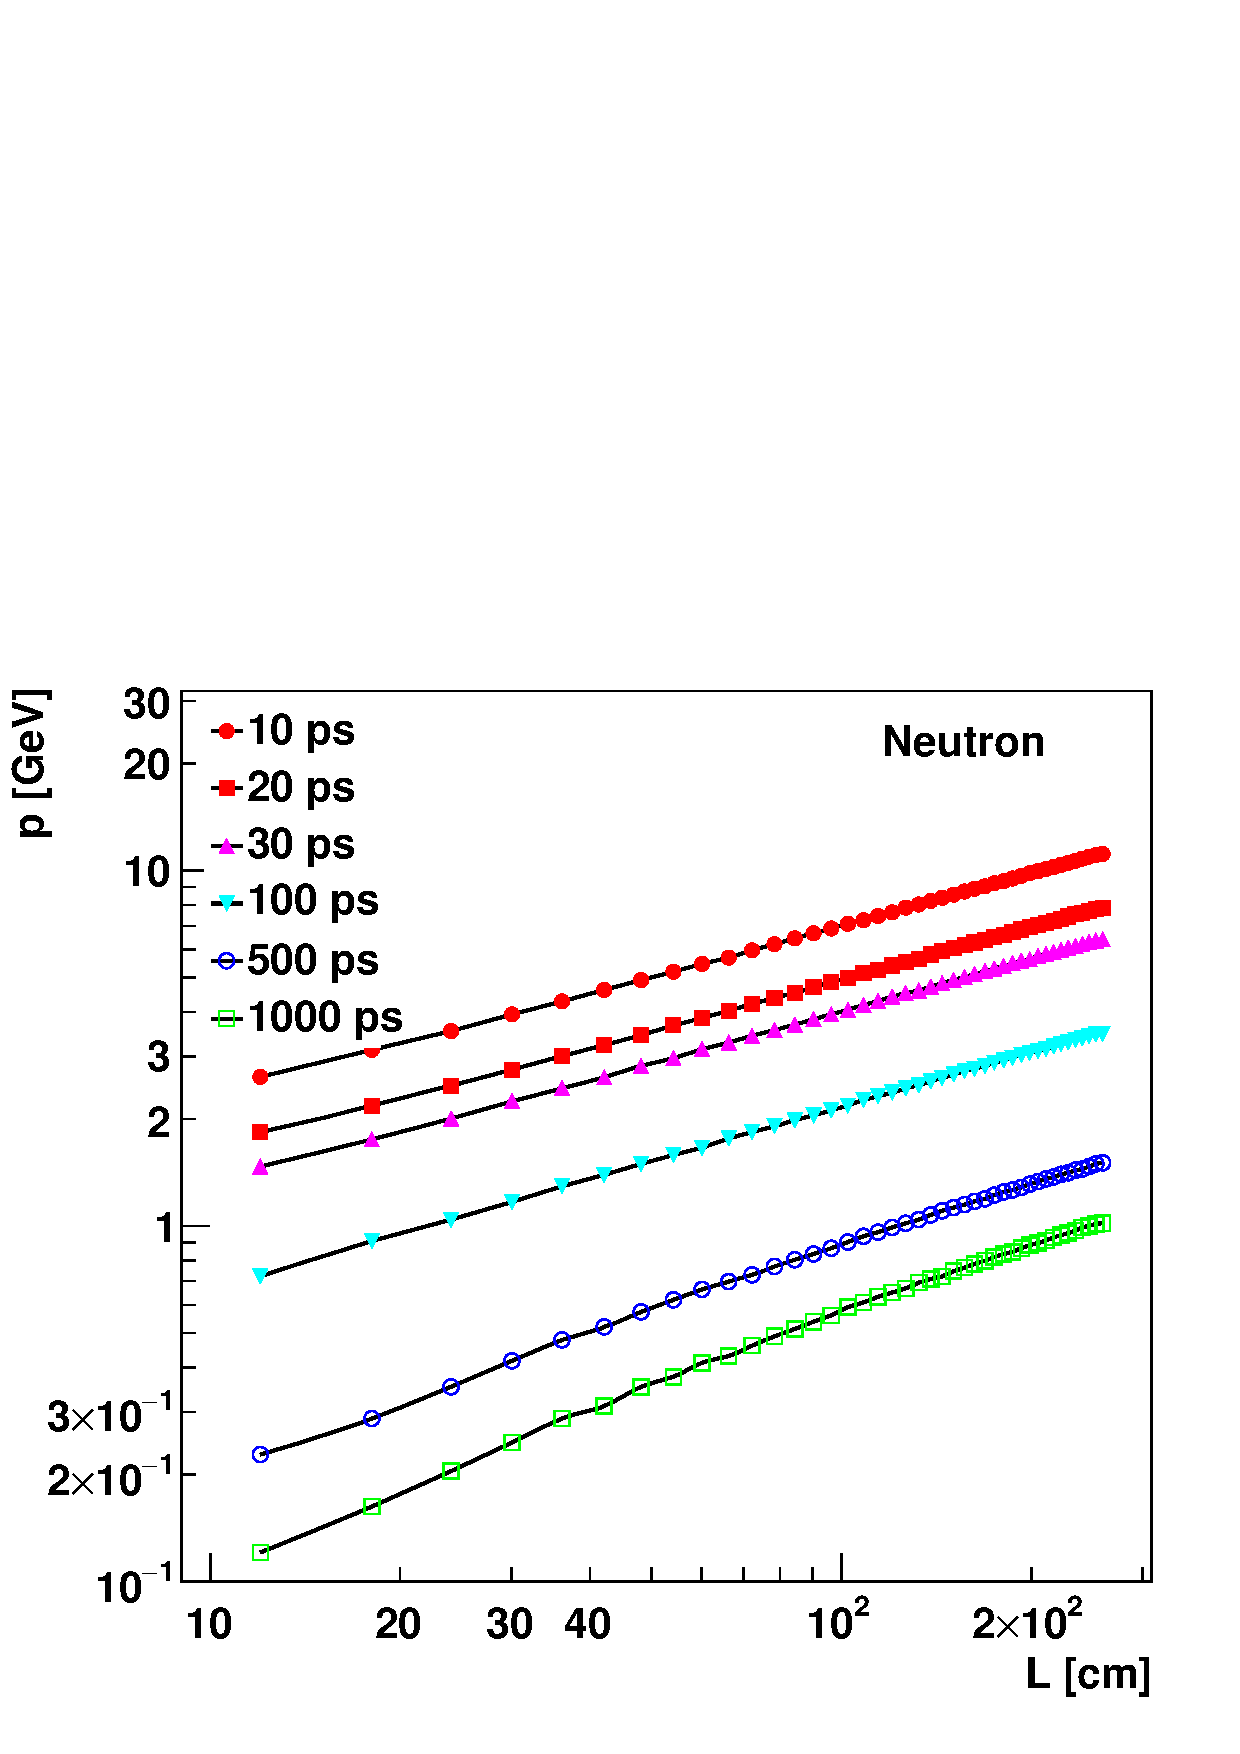
\includegraphics[width=0.45\textwidth]{time_flight_length_neutron.pdf}
   }
      \subfigure[$K$-mesons] {
   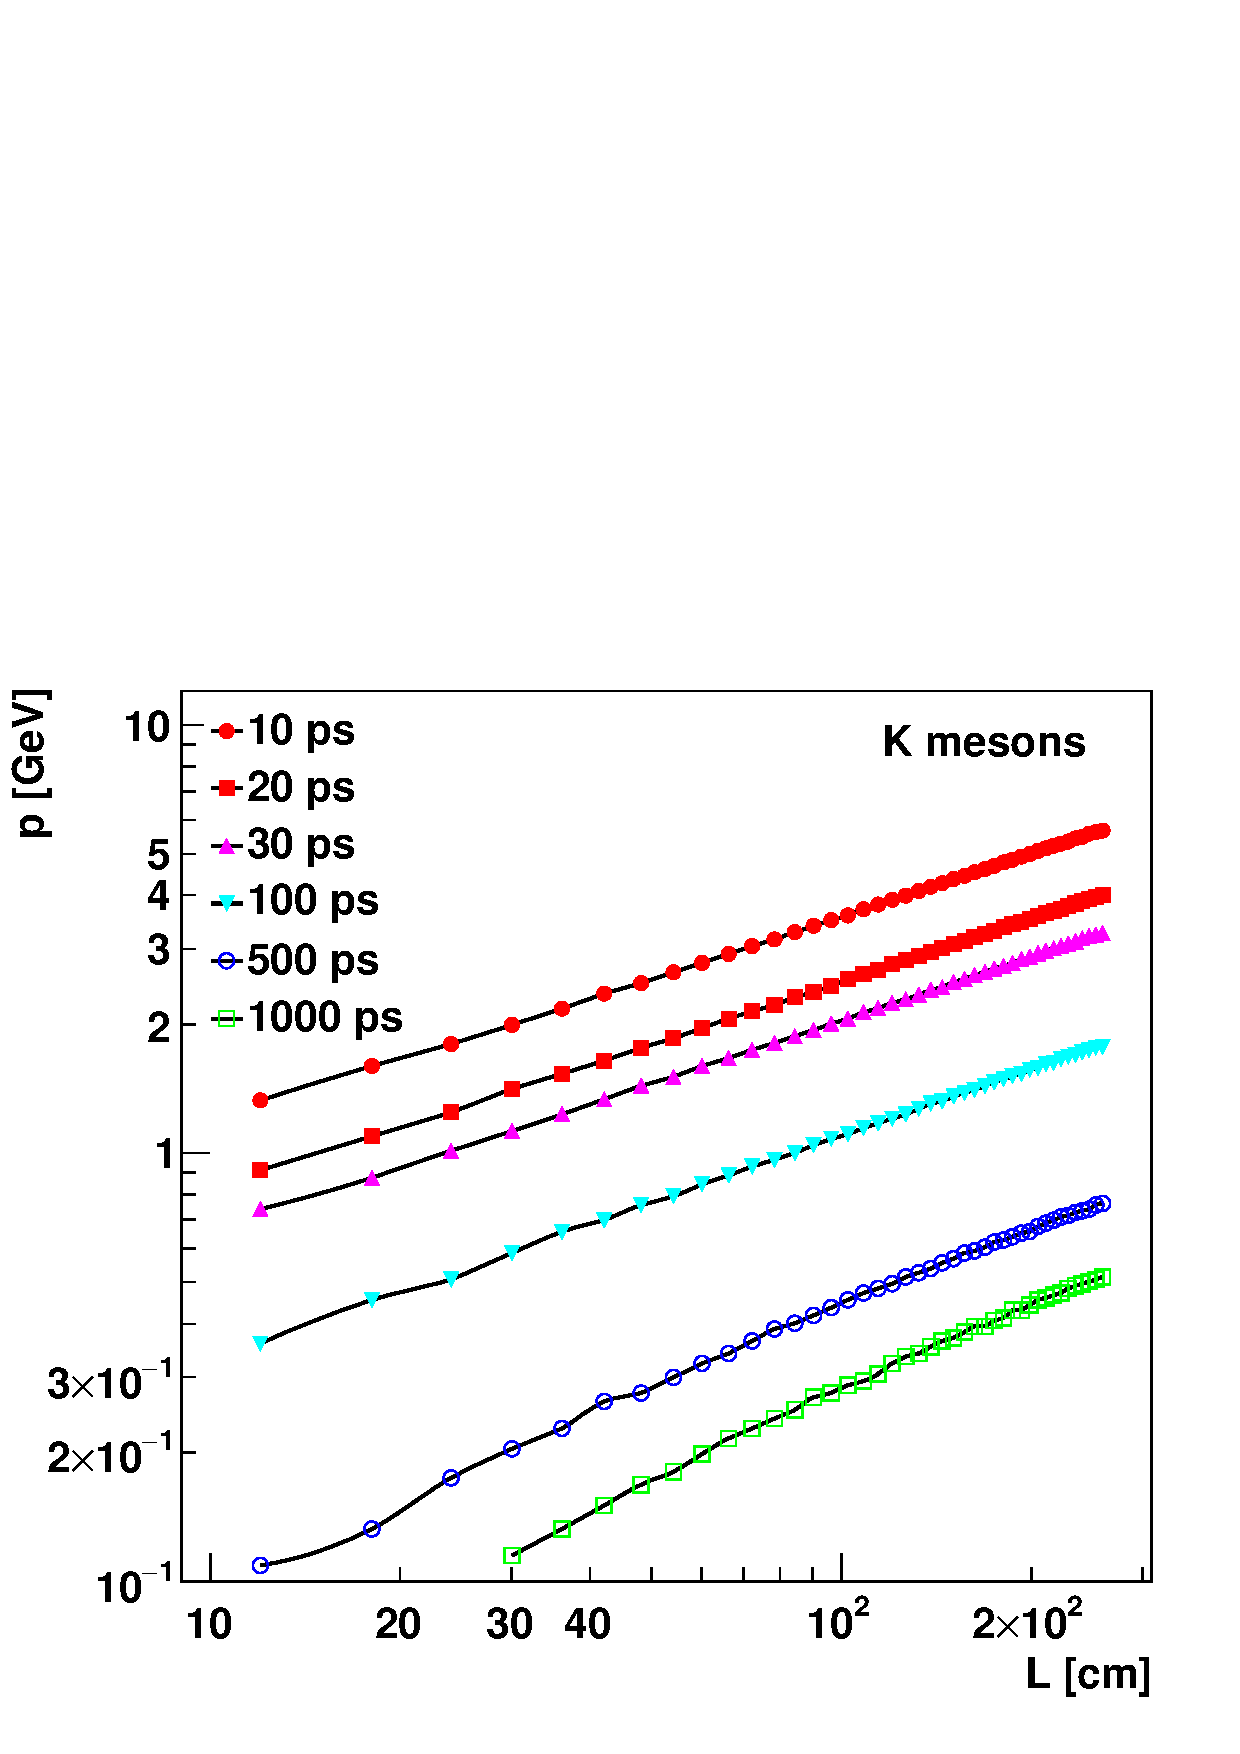
\includegraphics[width=0.45\textwidth]{time_flight_length_kion.pdf}\hfill
   }
\end{center}
\caption{
The $3\sigma$ separation from the pion mass hypothesis for neutrons and $K$-mesons as a function of the length of the particle's trajectory  $L$ and the momentum $p$.
For neutral particles the value of $L$ approximately corresponds the distance between the interaction point and the surface of the ECAL for $\eta=0$. 
}
\label{fig:singleparticles}
\end{figure}


\begin{figure}
\begin{center}
   \subfigure[for $L=2$~m] {
   \includegraphics[width=0.45\textwidth]{time_flight_200.pdf}
   }
   \subfigure[for $L=0.2$~m] {
   \includegraphics[width=0.45\textwidth]{time_flight_20.pdf}\hfill
   }
\end{center}
\caption{
The $3\sigma$ separation from $\alpha$ particles for heavy particles assuming timing layers with different resolutions for TOF, and using (a) $L=2$~m and (b) $L=0.2$~m.
The first value of $L$ approximately equals to a typical distance
from the interaction vertex to the first layer TL1, while the second value is the typical  distance
between two timing layers enclosing an electromagnetic calorimeter, assuming a typical calorimeter
based on the silicon technology.
}
\label{fig:signgleBSM}
\end{figure}


Having discussed a rather classical case of identification of neutrons (or protons) and the $K$-mesons from the pion hypothesis,
let us turn to the BSM searches for heavy particles.
The most abundant SM  background for light BSM  particles from primary interactions are protons and neutrons.
Other stable particles, that can be produced mainly in 
detector material (or in the interactions in the beam pipe) 
and detected by calorimeter are deuterons and $\alpha$ particles (composed of two protons and two neutrons). 
Although the rate of the $\alpha$ particles is  low since they can easily be stopped by detector material,
it is not impossible that the residual rate of such particle may still represent background for BSM searches that have a small production rate.  
Therefore, we will choose  $m_F=m_{\alpha}\simeq 3.73$~GeV  as a reference\footnote{We should emphasize that this choice of $\alpha$ particles for the reference mass scale  is
arbitrary and is only motivated by our attempt to check the $3\sigma$ separation in the momentum region $<10$~GeV.} in  Eq.~\ref{eqTOF}, and evaluate the
$3\sigma$ separation for a wide range of masses and momentum starting from 4~GeV.
For many planned experiments the distance between the 
interaction point and the first layer of the electromagnetic calorimeter is 
$1.5-2.5$~m. Therefore, for a representative purpose, we will use $L=2$~m and consider 0.2~m for the  separation
distance between the TL2 and TL1 timing layers.

Figure~\ref{fig:signgleBSM} shows the particle identification power for different choices of the timing layer resolution
and the travel distance $L$ (see Fig.~\ref{fig:eff_rad}).
For $L=2$~m, which approximately corresponds to the distance from the interaction point and 
the TL1 when a particle travels at $\eta=0$,  one can be see that a stable heavy particle with a mass of 100~GeV can be reconstructed up to 
400~GeV assuming a 20-ps timing layer,
but only up to 50~GeV using the standard 1-ns readout for time measurement.

In the case when  TOF is measured between the two layers, TL1 and TL2, assuming a successful spacial match of the hits,
the knowledge of the interaction vertex is not required.
This type of measurements can be beneficial
for neutral particles in collisions with large pile-up (multiple number of vertexes).
The identification power in the case when the travel distance $L=0.2$~m, i.e. when it  is close to the distance between TL2 and TL1, is shown in Figure~\ref{fig:signgleBSM}(b).
For a stable particle with a mass of 100~GeV, the identification is possible up to 100~GeV in momentum. The standard calorimeter with
$1$~ns resolution can only perform the identification up to $20$~GeV. 

